\chapter{Fundamentação teórica}

\section{Desenvolvimento de software} % (fold)
\label{sec:desenvolvimento_de_software}

O desenvolvimento de software é o ato de elaborar e implementar um sistema computacional que transforme as necessidades de um utilizador ou de um mercado em um produto de software.

O desenvolvimento de software é essencialmente uma atividade intelectual e criativa, exigindo a manipulação de uma gama muito grande de conhecimentos e informações. Além disso, além dos desenvolvedores de um software se preocuparem com o conteúdo e estrutura, eles devem se preocupar também com o comportamento fazendo com o que o desenvolvimento de software seja uma atividade complexa, devendo ser realizada por especialistas munidos de técnicas que os auxiliem da melhor maneira possível.

% section desenvolvimento_de_software (end)

\subsection{Agilismo} % (fold)
\label{sub:agilismo}

Em 2001 um grupo de dezessete especialistas, reconhecidos pela comunidade como grandes nomes do desenvolvimento software, se reuniram para discutir sobre um crescente conjunto de métodos que vinham surgindo e decidiram usar o termo Agilismo para descrever essa nova geração de métodos \cite{AgileStory}. Na mesma reunião, eles também escreveram o Manifesto Ágil \cite{AgileManifesto}, delineando um conjunto de valores e princípios que, em resumo, trilham um caminho para a eliminação de documentação e processos desnecessários, buscando a simplicidade, com foco na geração de valor e proximidade com o cliente, além de possibilitar respostas rápidas e eficazes às mudanças. Desde então, os métodos ágeis vêm ganhando projeção e importância no cenário da produção de software.

Pode-se dizer então, que o Desenvolvimento Ágil, ou Agilismo, é um rótulo genérico para os métodos de desenvolvimento de software baseados no Manifesto Ágil.

É importante citar que o desenvolvimento ágil sofreu grande influência de um conceito conhecido como \textit{Lean Thinking} (``pensamento enxuto"\ em português), uma linha de pensamento em gestão baseada nos princípios de \textit{Lean Manufacturing}\footnote{Os princípios de \textit{Lean Manufacturing} são originários do sistema Toyota de produção, que propôs um modo inteiramente novo de pensar a respeito de fabricação e logística de automóveis.} que se caracteriza por produção em pequenos lotes, eliminação de desperdícios, obsessão com qualidade, equipes multifuncionais praticando aprendizado contínuo, melhoria contínua de processo, sistema puxado de produção e a qualidade sendo responsabilidade dos trabalhadores como um todo \cite{BDDRodrigo}.

Uma das premissas do agilismo é que os custos de alterações sejam praticamente linear ao longo do tempo, independente do ponto em que esteja, fazendo com que a curva de custo de alterações seja semelhante à apresentada na Figura \ref{img:custo-agile}.

\begin{figure}[h]
  \center
  \caption{O custo das modificações no modelo ágil - Fonte: \cite{XPKent}}
  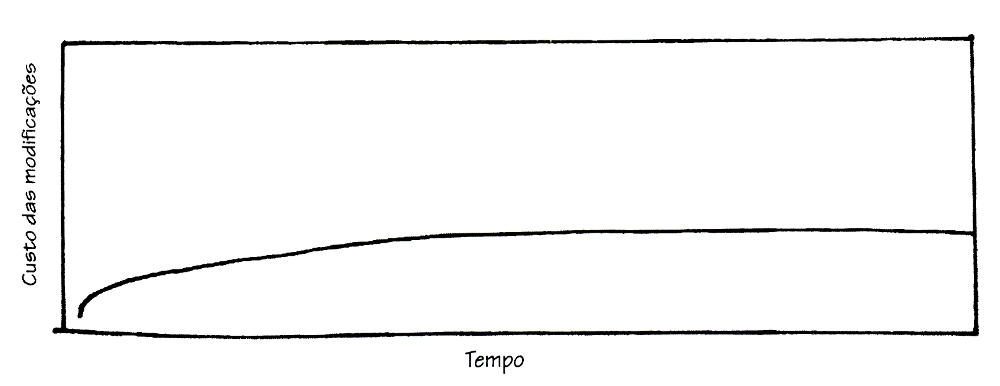
\includegraphics[scale=0.45]{images/custo-agile}
  \label{img:custo-agile}
\end{figure}

Isto é conseguido porque nos métodos ágeis não é feito um planejamento inicial muito abrangente. Ao invés disso, o desenvolvimento é dividido em iterações curtas (de uma a quatro semanas), onde ao início de cada uma delas é feito um novo planejamento, corrigindo o curso do projeto com base no \textit{feedback} obtido nas iterações anteriores. Para isso, a proximidade e interação do cliente com o projeto deve ser constante. Desta forma, o desenvolvimento é baseado em \textit{feedback} concreto e não em especulações sobre o futuro, fazendo com que o aprendizado permanente leve a melhorias e torne o produto final mais adequado para o seu público, além de o tornar mais simples e sem elementos extras que poderiam ser utilizados no futuro. Além disso, os testes automatizados são fundamentais para que as modificações realizadas não alterem o comportamento atual do sistema  \cite{XPKent}, dando segurança para que estas sejam feitas, além de permitir que o código melhore continuamente.

Ao utilizar métodos ágeis como \textit{eXtreme Programming} (XP) \nomenclature{XP}{eXtreme Programming} e Scrum, todas as funcionalidades do sistema são levantadas através de histórias, que são escritas pelo próprio cliente em pequenos cartões. A equipe de desenvolvimento utiliza os cartões para saber quais funcionalidades são desejadas pelo cliente. Contudo, os cartões podem acabar representando histórias que consomem muito esforço para serem implementadas. Nesse caso, a equipe divide os cartões em tarefas, que são registradas em novos cartões para serem distribuídas facilmente entre os desenvolvedores. Na Figura \ref{img:projeto_agile} é mostrada divisão de um projeto nos métodos ágeis.

\begin{figure}[h]
  \center
  \caption{Divisão de um projeto nos métodos ágeis}
  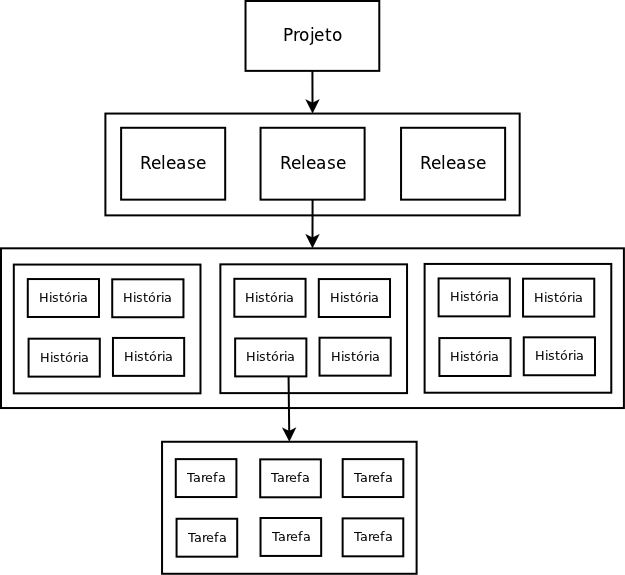
\includegraphics[scale=0.45]{images/projeto}
  \label{img:projeto_agile}
\end{figure}

No início do projeto o cliente e a equipe de desenvolvimento dividem o projeto em \textit{releases}, que são entregas de software que implementem um conjunto de funcionalidades que possui um valor bem definido para o cliente. Essas entregas são feitas de forma incremental, e em um espaço de tempo não muito longo (geralmente dois meses), para que o cliente possa começar a utilizar e obter os benefícios que elas oferecem, além de dar o \textit{feedback} necessário para que sejam feitas melhorias. Depois de definida a primeira \textit{release}, o cliente escreve as histórias que serão implementas nesta. As histórias das \textit{releases} posteriores podem ser deixadas para o futuro, pois durante o desenvolvimento de cada \textit{release} o cliente irá utilizar o software diversas vezes, o que irá influenciar as histórias das próximas \textit{release}. Durante a \textit{release} o cliente pode alterar as histórias se considerar necessário, podendo assim incorporar o aprendizado adquirido com o uso do sistema.

Uma \textit{release}, mesmo que seja pequena, representa um tempo ainda grande, pois não se deve esperar tanto tempo para ter o \textit{feedback} da utilização do software pelo cliente. Assim, ela é dividida em um conjunto de iterações, que são basicamente um pequeno espaço de tempo (geralmente duas semanas) dedicado para a implementação de um conjunto de histórias. A diferença entre uma \textit{release} e uma iteração é que na iteração o cliente não pode alterar as histórias definidas, pois a mudanças muito frequentes ao longo do trabalho da equipe de desenvolvimento prejudicam o ritmo de programação, pois confundem os desenvolvedores. No início de cara iteração é feita uma reunião para o planejamento da mesma, de modo que cliente e equipe de desenvolvimento definam as histórias que serão implementadas na iteração. Ao final de cada iteração e cada \textit{release}, o cliente tem novas histórias implementadas, ou seja, software funcionando. Dessa forma, ele poderá utilizar o sistema com as novas funcionalidades, tornando o \textit{feedback} ainda mais efetivo.

Mas para que isso seja possível, os métodos ágeis contam com um conjunto de técnicas para dar suporte a seu caráter iterativo e incremental, sendo algumas destas técnicas abordadas mais adiante neste trabalho.

% subsection agilismo (end)

% section desenvolvimento_de_software (end)

\section{Teste de software}
\label{sec:teste_de_software}


A maneira como o teste de software é aplicado varia de acordo com a metodologia utilizada no desenvolvimento. Tradicionalmente o teste de software é feito somente após o desenvolvimento ter sido concluído \cite{TesteSoftware, Pressman}. Já nos métodos ágeis um sentido oposto é seguido \cite{ArtOfAgileDevelopment}, sendo utilizadas técnicas como \textit{Test-Driven Development} (abordada na Seção \ref{sec:tdd}) e \textit{Behaviour-Driven Development} (abordada na Seção \ref{sec:bdd}).

O uso de estratégias nas quais a escrita dos testes automatizados é feita antes do código de implementação das funcionalidades, como TDD e BDD, não exclui o emprego de técnicas de teste de software tradicionais como classes de equivalência, análise do valor limite, análise da complexidade ciclomática e outras.

Os próximos tópicos definirão os tipos de teste utilizados no contexto do presente trabalho.

\subsection{Testes de unidade}
\label{sub:testes_de_unidade}

Testes de unidade são testes nos quais unidades individuais do sistema são testadas para determinar se estão aptas para uso. Uma unidade é a menor parte testável de uma aplicação. Em programação procedural uma unidade pode ser uma função. Já em programação orientada a objetos, uma unidade pode ser um método ou uma responsabilidade da classe. \citeonline{TesteSoftware} afirmam que neste contexto, espera-se que sejam identificados erros relacionados a algoritmos incorretos ou mal implementados, estruturas de dados incorretas, ou simplesmente erros de programação.

Para exemplificar, no Código \ref{code:unit_test_spec} é apresentado o teste de unidade para o método \texttt{Category\#name\_as\_css\_class}, cuja implementação é mostrada no Código \ref{code:unit_test}. Este método transforma o nome da Categoria em um nome de classe CSS\footnote{\textit{Cascading Style Sheets}. Mais em \url{http://pt.wikipedia.org/wiki/Cascading_Style_Sheets}}\nomenclature{CSS}{Cascading Style Sheets}, deixando todos seus caracteres em minúsculo e substituindo os caracteres / (barra),  (espaço) e - (traço) por \_ (sublinhado).

\begin{mycode}{rspec}%
{Teste de unidade automatizado para o método \texttt{Category\#name\_as\_css\_class} }{code:unit_test_spec}
# spec/models/category_spec.rb
describe Category do
  it "should return its name as a css class" do
    category = Factory.build :category, :name => "Feature"
    category.name_as_css_class.should == "feature"

    category.name = "New Feature"
    category.name_as_css_class.should == "new_feature"

    category.name = "Other-New Feature"
    category.name_as_css_class.should == "other_new_feature"

    category.name = "Study/Research"
    category.name_as_css_class.should == "study_research"
  end
end
\end{mycode}

\begin{mycode}{rspec}%
{Implementação do método \texttt{Category\#name\_as\_css\_class} }{code:unit_test}
# app/models/category.rb
class Category < ActiveRecord::Base
  def name_as_css_class
    self.name.downcase.gsub(/\/| |-/, "_")
  end
end
\end{mycode}

% subsection testes_de_unidade (end)

\subsection{Testes de integração}
\label{sub:testes_de_integracao}

No contexto do presente trabalho, os testes de integração testam as integrações do código com o mundo exterior. Eles podem ser testes que se comuniquem através da rede, tenham contato com o sistema de arquivos ou deixem os limites de seu próprio processo \cite{ArtOfAgileDevelopment}.

Para exemplificar, será utilizada uma extensão criada para fazer o destaque da sintaxe de código na descrição das Tarefas e no conteúdo do Comentários no kanban-roots, como apresentado na Figura \ref{img:highlighting}. Para isso, é utilizado um \textit{framework} em Python chamado Pygments\footnote{ Mais em \url{http://pygments.org/}}.

\begin{figure}[h]
  \center
  \caption{Comentário com destaque da sintaxe de código no kanban-roots}
  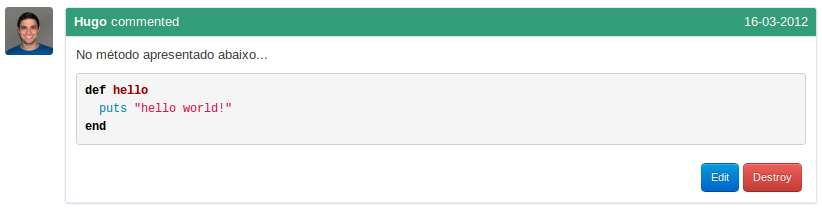
\includegraphics[scale=0.5]{images/highlighting}
  \label{img:highlighting}
\end{figure}

O Pygments deve ser instalado na máquina onde o kanban-roots está sendo executado. No entanto, o kanban-roots foi projetado rodar em um servidor próprio ou em um VPS\footnote{ \textit{Virtual Private Server}. É um servidor em ambiente compartilhado que possui acesso \textit{root} e processos independentes para cada conta VPS criada.}, mas também no Heroku\footnote{ É um PaaS (\textit{platafom as a service}) que tem uma cota de utilização gratuita. No Heroku não é possível instalar dependências no sistema. Mais em \url{http://heroku.com}}. Sendo assim, foi utilizado um serviço gratuito e não oficial criado por Trevor Turk e hospedado no Google App Engine que permite a utilização da API \nomenclature{API}{Application programming interface} do Pygments através de um POST para o serviço. Dessa forma, deve-se testar a integração com o serviço e também a integração com o Pygments instalado localmente.

\begin{mycode}{rspec}%
{Teste de integração automatizado para o \textit{highlighting} de código}{code:integration_spec}
# spec/lib/albino_render_spec.rb
describe HTMLwithAlbino do
  before(:all) do
    @render = HTMLwithAlbino.new
    @code_text = 'puts "hello!"'
    @highlighted_code =
      "<div class=\"highlight\"><pre>" +
        "<span class=\"nb\">puts</span> <span class=\"s2\">&quot;hello!&quot;</span>\n" +
      "</pre>\n</div>\n"
  end

  it "should get the highlighted block code from pygments.appspot.com" do
    @render.stub(:can_pygmentize?).and_return(false)
    @render.block_code(@code_text, "ruby").should == @highlighted_code
  end

  it "should get the highlighted block code from local pygments" do
    @render.stub(:can_pygmentize?).and_return(true)
    @render.block_code(@code_text, "ruby").should == @highlighted_code
  end
end
\end{mycode}

\begin{mycode}{ruby}%
{Implementação do \textit{highlighting} de código}{code:integration}
# lib/albino_render.rb
class HTMLwithAlbino < Redcarpet::Render::HTML
  def block_code(code, lang)
    if can_pygmentize?
      Albino.colorize(code, lang)
    else
      # This is a hack for pygments work on Heroku
      require "net/http"
      Net::HTTP.post_form(URI.parse("http://pygments.appspot.com/"),
                          {"code"=>code, "lang"=>lang}).body
    end
  end

  private
  def can_pygmentize?
    system "pygmentize -V"
  end
end
\end{mycode}

É importante perceber que, para isolar o \hyperref[code:integration_spec]{teste}, foi utilizado um dublê de teste (neste caso um \textit{stub}) para simular a resposta do método \texttt{can\_pygmentize?} que faz uma verificação no sistema operacional para verificar se o Pygments está instalado ou não. Dublês de teste serão abordados mais detalhadamente na Seção \ref{sec:dubles_de_teste}.

% subsection testes_de_integracao (end)

\subsection{Testes de aceitação}
\label{ssub:testes_de_aceitacao}

Testes de aceitação são especificações para o comportamento das funcionalidades de um sistema. Eles mostram se o sistema se comporta corretamente pela perspectiva de um usuário, sem nos dizer nada sobre como o sistema implementa esse comportamento \cite{TestDrivenKoskela}. Além disso, é verificada a integração entre as diversas unidades que interagem para prover esta funcionalidade.

Relacionando com os métodos tradicionais, os testes de aceitação implementam os casos de uso levantados na análise orientada a objetos.

No Código \ref{code:acceptance} são apresentados exemplos de teste de aceitação, sendo dois cenários de uma mesma funcionalidade, utilizando BDD com a escrita testes em texto plano. BDD e testes de aceitação serão vistos com mais detalhes na Seção \ref{sec:bdd}.

\begin{mycode}{cucumber}%
{Teste de aceitação para o registro de um contribuidor}{code:acceptance}
# features/board.feature
Feature: Use the board
  As a user
  I want use the board
  In order see, move and manipulate the taks of my project

  @javascript
  Scenario: Drag and drop a task to another board position
    Given I am an authenticated contributor
    And I have a project
    And the following tasks:
      | title  | position |
      | task 1 | Doing    |
      | task 2 | Done     |
    And I am on the projects board page
    When I drag "task 1" task to "Done" position
    Then I should see "task 1" task at "Done" position

  Scenario: Clean up Done tasks
    Given I am an authenticated contributor
    And I have a project
    And the following tasks:
      | title  | position |
      | task 1 | Doing    |
      | task 2 | Done     |
      | task 3 | Done     |
      | task 4 | Done     |
    When I am on the projects board page
    And I follow "Clean up Done"
    Then I should see "Done division was cleaned up."
    And the Done division should be cleaned
\end{mycode}

% subsection testes_de_aceitacao (end)

% section teste_de_software (end)

